\item Se selecciona un punto al azar en el interior de un círculo. Hallar la probabilidad de que el punto quede más cercano al centro que a la circunferencia.\e\\
    Se tiene la siguiente situación
    \begin{center}
        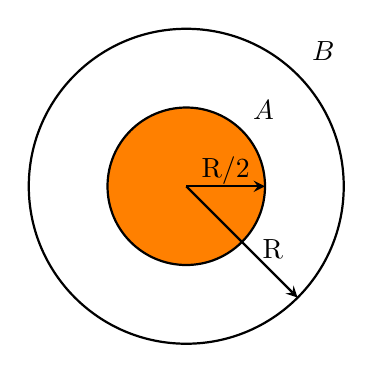
\begin{tikzpicture}
            [thick,
            set/.style = {circle,
                        minimum size = 2cm}]
            \fill[orange] (0,0) circle (1);
            \node[set,label={45:$A$}] (A) at (0,0) {};
            \node[set,label={45:$B$}] (B) at (0.75,0.75) {};
            % Dibujo conjuntos
            \draw (0,0) circle(1cm);
            \draw (0,0) circle(2cm);
            \draw [-stealth](0,0) -- (1,0);
            \draw [-stealth](0,0) -- (1.414,-1.414);

            \node at (0.5,0.2) {R/2};
            \node at (1.1,-0.8) {R};
        \end{tikzpicture}
    \end{center}
    En donde A es el área de interés, mientras que B es el área total. Entonces,
    \[P(A)=\frac{\text{área }A}{\text{área }B}=\frac{\pi \cdot (R/2)^2}{\pi\cdot R^2}=\frac{1}{4}\]